\begin{figure}
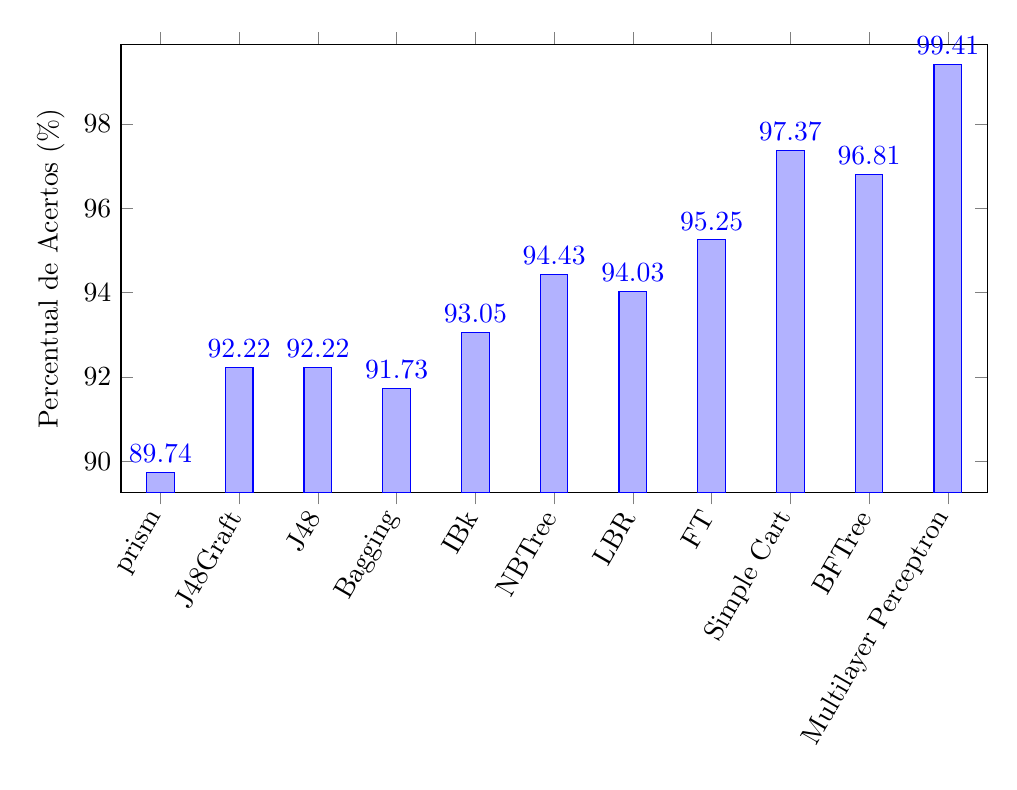
\begin{tikzpicture} \begin{axis}[
    ybar, x=1cm,
    enlargelimits=0.05,
    legend style={at={(0.5,-0.2)},
    anchor=north,legend columns=-1},
    ylabel={Percentual de Acertos (\%)},
    symbolic x coords={prism,J48Graft,J48,%
     Bagging,IBk, NBTree, LBR, FT, Simple Cart, BFTree, Multilayer Perceptron},
     xtick=data,
     nodes near coords, nodes near coords align={vertical},
    x tick label style={rotate=60,anchor=east}, ]
\addplot coordinates {(prism,89.74) (J48Graft,92.22) (J48,92.22) (Bagging,91.73) (IBk,93.05) (NBTree,94.43) (LBR, 94.03)
    (FT, 95.25) (Simple Cart, 97.37) (BFTree, 96.81) (Multilayer Perceptron, 99.41) };
\end{axis}
\end{tikzpicture}
\caption{Ranking do percentual de acerto dos algoritmos}
\label{figure:ranking}
\end{figure}

\begin{table}[h]
  \begin{center}
    \begin{tabular}{ l | l | l | l}
      \hline
      Domínio & Instâncias & Atributos & Tipo de Classe \\ \hline
      Bresat Cancer Winscosin & 699 & 9 & Discreta \\ \hline
    \end{tabular}
    \caption[Dados do domínio]{Dados do conjunto de dados Breast Cancer Winscosin\cite{donator:92}}
    \label{table:dataset}
  \end{center}
\end{table}

\begin{table}
  \begin{center}
    \begin{tabular}{ l | l }
      \hline
      \multicolumn{2}{c}{ \bfseries Base do Hospital de Winscosin} \\ \hline
      \bfseries Atributo & \bfseries Intervalo inteiro\\ \hline
      Clump Thickness & Entre 1 e 10 \\
      Uniformity of Cell Size & Entre 1 e 10 \\
      Uniformity of Cell Shape & Entre 1 e 10 \\
      Marginal Adhesion & Entre 1 e 10 \\
      Single Epithelial Cell Size & Entre 1 e 10 \\
      Bare Nuclei & Entre 1 e 10 \\
      Bland Chromatin & Entre 1 e 10 \\
      Normal Nucleoli & Entre 1 e 10 \\
      Mitoses & Entre 1 e 10 \\
      \hline
    \end{tabular}
  \end{center}
  \caption{ As classes são escritas como 2 para beníngo e 4 para malígno}
  \label{table:disposicao-atributos}
\end{table}

\begin{table}
  \begin{center}
    \begin{tabular}{ l | l }
      \hline
      \multicolumn{2}{c}{ \bfseries Algoritmos de Classificação} \\ \hline
      \bfseries Método & \bfseries Tipo \\ \hline
      Multilayer Perceptron & Função \\
      SimpleCart & Árvore \\
      J48graft & Árvore \\
      J48 & Árvore \\
      Bagging & Meta \\
      BFTree & Árvore \\
      FT & Árvore \\
      NBTree & Árvore \\
      Prism & Regras \\
      IBk & Lazy \\
      LBR & Lazy \\
      \hline
    \end{tabular}
  \end{center}
  \caption{Os 11 algoritmos selecionados para realizar as comparações.}
  \label{table:algoritmos}
\end{table}


\begin{table}
  \begin{center}
    \begin{tabular}{ l | l  l  l}
      \hline
      \multicolumn{3}{c}{\bfseries Comparações do algoritmo multilayer perceptron } \\ \hline
      Algoritmo & Percentual de acerto & Raiz do erro quadrado &Tempo \\ \hline
       (1) Multilayer Perceptron & 99.41 & 0.04327 & 0.00081  \\
       (2) Simple Cart & 97.37 * & 0.10374 v & 0.00010 * \\
       (3) J48Graft & 92.22 * & 0.16656 v &0.00009 * \\
       (4) J48 & 92.22 * & 0.16656 v &0.00015 *\\
      (5) Bagging & 91.73 * & 0.16951 v & 0.00032 *  \\
      (6) BFTree  & 96.81 * & 0.10832 v & 0.00012 * \\
      (7) FT  & 95.25 * & 0.13906 v& 0.01839 v \\
      (8) NBTree & 94.43 * & 0.15783 v & 0.00180 v\\
      (9) Prism  & 89.74 * & 0.13245 v & 0.00029 * \\
      (10) IBk  & 93.05 * & 0.19608 v & 0.01454 v \\
      (11) LBR  & 94.03 * & 0.17340 v & 0.26227 v\\ \hline
    \end{tabular}
  \end{center}
\caption{Resultados da comparação do Multilayer Perceptron com os demais algoritmos.
  Os resultados que apresentam um *, indicam que foram significantemente menores,
  enquanto os que apresentam um \emph{v}, indicam que foram significantemente maiores.
  Os resultados que não apresentam nenhum símbolo ao seu lado, foram significantemente
  iguais.}
\label{table:results}
\end{table}
